%=============================================================================
% IRS Phase Shift Optimization - Research Report
%=============================================================================
\documentclass[12pt,a4paper]{article}

% ---- Packages ----
\usepackage[utf8]{inputenc}
\usepackage[T1]{fontenc}
\usepackage[english]{babel}
\usepackage{amsmath,amssymb,amsfonts}
\usepackage{mathtools}
\usepackage{graphicx}
\usepackage{float}
\usepackage{booktabs}
\usepackage{caption}
\usepackage{subcaption}
\usepackage[margin=2.5cm]{geometry}
\usepackage{algorithm}
\usepackage{algorithmic}
\usepackage{cite}
\usepackage{url}
\usepackage{array}
\usepackage{multirow}
\usepackage{tabularx}
\usepackage{enumitem}
\usepackage{xcolor}
\usepackage{fancyhdr}
\usepackage{setspace}
\usepackage{tikz}
\usepackage{parskip}

% ---- Must load hyperref AFTER most packages, cleveref AFTER hyperref ----
\usepackage{hyperref}
\usepackage{cleveref}

% ---- Page style ----
\pagestyle{fancy}
\fancyhf{}
\fancyhead[R]{\thepage}
\fancyhead[L]{\textit{IRS Phase Shift Optimization}}
\renewcommand{\headrulewidth}{0.4pt}

% ---- Hyperref setup: black links for TOC/LOF, colored for citations ----
\hypersetup{
    colorlinks=true,
    linkcolor=black,
    citecolor=green!50!black,
    urlcolor=cyan!60!black,
}

% ---- Spacing ----
\setlength{\parskip}{6pt}
\setlength{\parindent}{0pt}

% ---- Custom commands ----
\newcommand{\vect}[1]{\boldsymbol{#1}}
\newcommand{\mat}[1]{\mathbf{#1}}
\newcommand{\abs}[1]{\left|#1\right|}
\newcommand{\norm}[1]{\left\|#1\right\|}
\DeclareMathOperator*{\argmax}{arg\,max}
\DeclareMathOperator*{\argmin}{arg\,min}
\DeclareMathOperator{\diag}{diag}
\DeclareMathOperator{\tr}{tr}

%=============================================================================
\begin{document}

%=============================================================================
% TITLE PAGE
%=============================================================================
\begin{titlepage}
\centering
\vspace*{4cm}

{\LARGE \textbf{Maximizing Achievable Data Rate in}}\\[0.4cm]
{\LARGE \textbf{Intelligent Reflecting Surface-Aided}}\\[0.4cm]
{\LARGE \textbf{Wireless Communication Systems}}\\[1.2cm]

\rule{0.6\textwidth}{0.8pt}\\[1.2cm]

{\large Phase-Level, Component-Level, and Hybrid\\[0.2cm]
Optimization Using Metaheuristic Algorithms}\\[2cm]

\vfill

{\large 2026}
\end{titlepage}

%=============================================================================
% TABLE OF CONTENTS
%=============================================================================
\newpage
\tableofcontents
\newpage
\listoffigures
\listoftables
\newpage

%=============================================================================
% 1. INTRODUCTION
%=============================================================================
\section{Introduction}
\label{sec:introduction}

\subsection{Background and Motivation}

Intelligent Reflecting Surfaces (IRS) have emerged as one of the most promising technologies for next-generation wireless communication systems \cite{wu2020towards, huang2019reconfigurable}. An IRS consists of a large number of low-cost passive reflecting elements, each of which can independently adjust the phase shift of the incident signal, thereby collaboratively creating favorable propagation conditions. Unlike traditional relay-based approaches, IRS operates without requiring dedicated radio frequency (RF) chains, power amplifiers, or signal processing hardware, making it a cost-effective and energy-efficient solution for enhancing wireless coverage and capacity \cite{wu2019intelligent}.

The fundamental principle behind IRS technology is the ability to constructively combine reflected signals with the direct path signal at the user equipment (UE). By carefully optimizing the phase shifts of all reflecting elements, the IRS can maximize the signal-to-noise ratio (SNR) at the receiver, leading to significant improvements in the achievable data rate. The optimization of these phase shifts, however, is a highly non-convex problem, particularly when considering practical hardware constraints \cite{abeywickrama2020intelligent}.

\subsection{The Ideal vs. Practical Phase Shift Model}

Most existing works on IRS phase shift optimization assume an \textit{ideal} reflection model, where each reflecting element can independently adjust its phase shift $\theta_n \in [-\pi, \pi]$ while maintaining unit reflection amplitude, i.e., $|v_n| = 1$. Under this ideal assumption, the reflection coefficient of the $n$-th element is simply:
\begin{equation}
    v_n = e^{j\theta_n}, \quad \theta_n \in [-\pi, \pi].
    \label{eq:ideal_model}
\end{equation}

However, in practical IRS hardware, the reflection amplitude $\beta_n(\theta_n)$ is inherently coupled with the phase shift $\theta_n$ due to physical limitations of the circuit components (e.g., varactor diodes) \cite{abeywickrama2020intelligent}. This amplitude-phase coupling means that the reflection coefficient has a phase-dependent amplitude:
\begin{equation}
    v_n = \beta_n(\theta_n) e^{j\theta_n}, \quad \theta_n \in [-\pi, \pi], \quad \beta_n(\theta_n) \in [\beta_{\min}, 1].
    \label{eq:practical_model}
\end{equation}

Ignoring this coupling during the design phase leads to sub-optimal performance, as the actual reflected signal amplitude differs from the assumed unit amplitude. This research addresses the performance gap between ideal and practical models and develops optimization algorithms that directly account for the amplitude-phase coupling.

\subsection{Research Objectives}

This research pursues the following objectives:
\begin{enumerate}[label=(\roman*)]
    \item \textbf{Phase-level optimization:} Optimize the continuous phase shift vector $\vect{\theta} = [\theta_1, \theta_2, \ldots, \theta_N]^T$ under both the ideal and practical reflection models using analytical methods (Alternating Optimization) and metaheuristic algorithms (PSO, GWO).

    \item \textbf{Component-level optimization:} Directly optimize the hardware circuit parameters $\{L_{1,n}, L_{2,n}, C_n, R_n\}$ of each IRS element to maximize the achievable rate, accounting for the full electromagnetic behavior of the circuit.

    \item \textbf{Hybrid optimization:} Combine phase-level and component-level optimization through a warm-started approach that uses the analytical phase-level solution to guide the component-level search.

    \item \textbf{Comprehensive comparison:} Compare the performance, convergence behavior, and computational cost of all proposed approaches through extensive Monte Carlo simulations.
\end{enumerate}

\subsection{Paper Organization}

The remainder of this report is organized as follows. Section~\ref{sec:system_model} presents the system model including the channel model, the practical phase shift model, and the circuit impedance model. Section~\ref{sec:problem_formulation} formulates the optimization problems at both the phase level and the component level. Section~\ref{sec:algorithms} describes all optimization algorithms including AO, PSO, GWO, and the hybrid approaches. Section~\ref{sec:simulation} details the simulation setup and experimental methodology. Section~\ref{sec:results} presents and discusses the numerical results. Finally, Section~\ref{sec:conclusion} concludes the report.


%=============================================================================
% 2. SYSTEM MODEL
%=============================================================================
\section{System Model}
\label{sec:system_model}

\subsection{IRS-Aided Wireless Communication System}

We consider a single-user multiple-input single-output (MISO) system where an access point (AP) equipped with $M = 2$ antennas serves a single-antenna user with the assistance of an IRS consisting of $N$ reflecting elements, as illustrated in \Cref{fig:system_model}. The IRS is deployed between the AP and the user to establish a strong reflected link, thereby enhancing the received signal quality.

\begin{figure}[htbp]
    \centering
    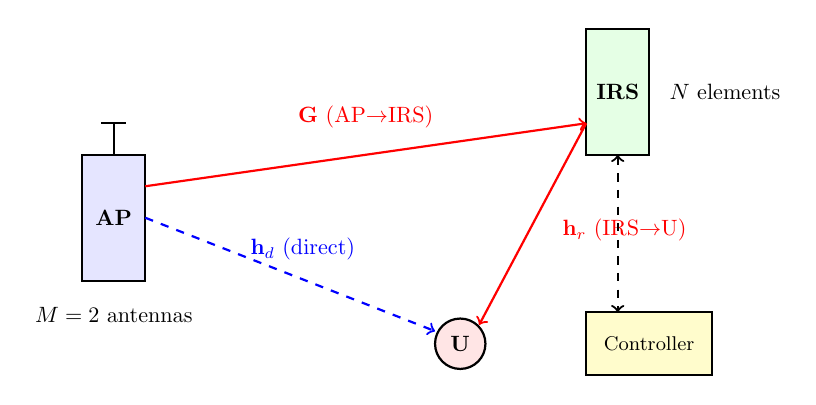
\begin{tikzpicture}[scale=0.8, every node/.style={scale=0.8}]
        % AP
        \draw[thick, fill=blue!10] (0,0) rectangle (1,2);
        \node at (0.5,1) {\textbf{AP}};
        \draw[thick] (0.5,2) -- (0.5,2.5);
        \draw[thick] (0.3,2.5) -- (0.7,2.5);
        \node[below] at (0.5,-0.3) {$M=2$ antennas};

        % IRS
        \draw[thick, fill=green!10] (8,2) rectangle (9,4);
        \node at (8.5,3) {\textbf{IRS}};
        \node[right] at (9.2,3) {$N$ elements};

        % User
        \draw[thick, fill=red!10] (6,-1) circle (0.4);
        \node at (6,-1) {\textbf{U}};

        % Direct link
        \draw[->, thick, blue, dashed] (1,1) -- (5.6,-0.8);
        \node[blue] at (3.5,0.5) {$\mat{h}_d$ (direct)};

        % AP to IRS link
        \draw[->, thick, red] (1,1.5) -- (8,2.5);
        \node[red, above] at (4.5,2.3) {$\mat{G}$ (AP$\to$IRS)};

        % IRS to User link
        \draw[->, thick, red] (8,2.5) -- (6.3,-0.7);
        \node[red, right] at (7.5,0.8) {$\mat{h}_r$ (IRS$\to$U)};

        % IRS Controller
        \draw[thick, fill=yellow!20] (8,-1.5) rectangle (10,-0.5);
        \node at (9,-1) {\small Controller};
        \draw[<->, thick, dashed] (8.5,2) -- (8.5,-0.5);
    \end{tikzpicture}
    \caption{An IRS-aided MISO wireless communication system. The AP transmits signals to the user through both the direct link $\mat{h}_d$ and the reflected link via the IRS. The IRS controller adjusts the phase shifts of the $N$ reflecting elements.}
    \label{fig:system_model}
\end{figure}

\subsection{Channel Model}

The system involves three wireless links, each modeled with Rayleigh fading and distance-dependent path loss:

\begin{itemize}
    \item \textbf{AP$\to$User (direct link):} $\mat{h}_d \in \mathbb{C}^{M \times 1}$, with path loss exponent $\alpha_{AU} = 3.8$.
    \item \textbf{AP$\to$IRS:} $\mat{G} \in \mathbb{C}^{N \times M}$, with path loss exponent $\alpha_{AI} = 2.2$.
    \item \textbf{IRS$\to$User:} $\mat{h}_r \in \mathbb{C}^{N \times 1}$, with path loss exponent $\alpha_{IU} = 2.8$.
\end{itemize}

The path loss at distance $d$ is given by:
\begin{equation}
    \text{PL}(d) = C_0 \cdot d^{-\alpha},
    \label{eq:path_loss}
\end{equation}
where $C_0 = 10^{-4}$ ($-40$~dB reference path loss at 1~m) and $\alpha$ is the path loss exponent.

Each channel is generated as:
\begin{equation}
    \mat{h} = \sqrt{\frac{\text{PL}(d)}{2}} \left(\mat{h}_{\text{real}} + j\mat{h}_{\text{imag}}\right),
\end{equation}
where $\mat{h}_{\text{real}}$ and $\mat{h}_{\text{imag}}$ are independent standard normal random vectors.

\subsubsection{Geometry}

The geometry of the system is defined as follows:
\begin{itemize}
    \item The AP is located at the origin $(0, 0)$.
    \item The IRS is located at $(D_{AP\text{-}IRS}, 0) = (500, 0)$~m.
    \item The user is located at $(d_{\text{horizontal}}, D_{\text{vertical}}) = (d, 2)$~m, where $d$ is varied.
\end{itemize}

The link distances are computed as:
\begin{align}
    d_{AU} &= \sqrt{d^2 + D_{\text{vertical}}^2}, \\
    d_{IU} &= \sqrt{(D_{AP\text{-}IRS} - d)^2 + D_{\text{vertical}}^2}, \\
    d_{AI} &= D_{AP\text{-}IRS} = 500 \text{ m}.
\end{align}

The combined channel matrix is defined as:
\begin{equation}
    \mat{\Phi} = \diag(\mat{h}_r^H) \mat{G} \in \mathbb{C}^{N \times M}.
    \label{eq:combined_channel}
\end{equation}

\subsection{Signal Model and Achievable Rate}

With maximum ratio transmission (MRT) beamforming at the AP, the achievable rate (spectral efficiency) in bits/s/Hz is:
\begin{equation}
    R_{SE} = \log_2\left(1 + \frac{P_T}{\sigma^2} \norm{\vect{v}^H \mat{\Phi} + \mat{h}_d^H}^2\right),
    \label{eq:achievable_rate}
\end{equation}
where $P_T$ is the transmit power, $\sigma^2$ is the noise power, and $\vect{v} \in \mathbb{C}^N$ is the IRS reflection coefficient vector.

The channel gain, which is the key quantity to maximize, is:
\begin{equation}
    F(\vect{v}) = \norm{\vect{v}^H \mat{\Phi} + \mat{h}_d^H}^2.
    \label{eq:channel_gain}
\end{equation}

Since $R_{SE}$ is a strictly increasing function of $F(\vect{v})$, maximizing the channel gain is equivalent to maximizing the achievable rate.

\subsection{Practical Phase Shift Model}
\label{sec:practical_model}

Following the model proposed by Abeywickrama et al.\ \cite{abeywickrama2020intelligent}, the phase-dependent reflection amplitude is:
\begin{equation}
    \beta(\theta_n) = (1 - \beta_{\min}) \left(\frac{\sin(\theta_n - \phi) + 1}{2}\right)^k + \beta_{\min},
    \label{eq:beta_model}
\end{equation}
where the model parameters, fitted from measured varactor-based IRS prototypes, are:
\begin{itemize}
    \item $\beta_{\min} = 0.2$: minimum reflection amplitude,
    \item $\phi = 0.43\pi$: horizontal shift of the amplitude curve,
    \item $k = 1.6$: steepness parameter controlling the curve shape.
\end{itemize}

The practical reflection coefficient for the $n$-th element is then:
\begin{equation}
    v_n = \beta(\theta_n) e^{j\theta_n}, \quad \theta_n \in [-\pi, \pi], \quad \beta(\theta_n) \in [\beta_{\min}, 1].
    \label{eq:reflection_coeff}
\end{equation}

Note that when $k = 0$, $\beta(\theta_n) = 1$ for all $\theta_n$, reducing to the ideal model. As $k$ increases, the amplitude-phase coupling becomes more pronounced.

\subsection{Circuit Impedance Model}
\label{sec:circuit_model}

Each IRS reflecting element is modeled as a parallel resonant circuit consisting of four hardware components:
\begin{itemize}
    \item $L_{1,n}$: coupling inductance ($0.5$--$5.0$ nH),
    \item $L_{2,n}$: varactor series inductance ($0.1$--$3.0$ nH),
    \item $C_n$: varactor capacitance ($0.1$--$5.0$ pF),
    \item $R_n$: varactor equivalent series resistance ($0.5$--$5.0$ $\Omega$).
\end{itemize}

The equivalent impedance of the $n$-th element at operating frequency $f = 5.8$~GHz ($\omega = 2\pi f$) is \cite{abeywickrama2020intelligent}:
\begin{equation}
    Z_n = \frac{j\omega L_{1,n} \left(j\omega L_{2,n} + \frac{1}{j\omega C_n} + R_n\right)}{j\omega L_{1,n} + j\omega L_{2,n} + \frac{1}{j\omega C_n} + R_n}.
    \label{eq:impedance}
\end{equation}

The reflection coefficient is then determined by the impedance mismatch with the free-space impedance $Z_0 \approx 377~\Omega$:
\begin{equation}
    v_n = \frac{Z_n - Z_0}{Z_n + Z_0}.
    \label{eq:reflection_from_impedance}
\end{equation}

The resulting $v_n$ is a complex number with both amplitude $|v_n|$ and phase $\arg(v_n)$ constrained by the physical circuit parameters. This means that unlike the phase-level formulation where the reflection amplitude follows a deterministic model of \eqref{eq:beta_model}, the component-level formulation captures the full electromagnetic behavior of the hardware.


%=============================================================================
% 3. PROBLEM FORMULATION
%=============================================================================
\section{Problem Formulation}
\label{sec:problem_formulation}

\subsection{Phase-Level Optimization}

The phase-level optimization problem seeks to find the optimal phase shift vector $\vect{\theta} = [\theta_1, \theta_2, \ldots, \theta_N]^T$ that maximizes the achievable rate:
\begin{equation}
    \begin{aligned}
        \max_{\vect{\theta}} \quad & R_{SE} = \log_2\left(1 + \frac{P_T}{\sigma^2} \norm{\vect{v}^H \mat{\Phi} + \mat{h}_d^H}^2\right) \\
        \text{s.t.} \quad & \theta_n \in [-\pi, \pi], \quad n = 1, \ldots, N, \\
        & v_n = \beta(\theta_n) e^{j\theta_n}, \quad \text{(practical model)}, \\
        & \text{or } v_n = e^{j\theta_n}, \quad \text{(ideal model)}.
    \end{aligned}
    \label{eq:phase_optimization}
\end{equation}

This problem is non-convex due to the non-linear dependence of $R_{SE}$ on $\vect{\theta}$, compounded by the amplitude-phase coupling in the practical model.

\subsection{Component-Level Optimization}

The component-level optimization directly searches over the hardware parameter space:
\begin{equation}
    \begin{aligned}
        \max_{\mat{x}} \quad & R_{SE} = \log_2\left(1 + \frac{P_T}{\sigma^2} \norm{\vect{v}^H \mat{\Phi} + \mat{h}_d^H}^2\right) \\
        \text{s.t.} \quad & \mat{x}_n = [L_{1,n},\, L_{2,n},\, C_n,\, R_n]^T, \\
        & \mat{x} = [\mat{x}_1^T,\, \mat{x}_2^T,\, \ldots,\, \mat{x}_N^T]^T \in \mathbb{R}^{4N}, \\
        & L_{1,n} \in [0.5, 5.0] \text{ nH}, \\
        & L_{2,n} \in [0.1, 3.0] \text{ nH}, \\
        & C_n \in [0.1, 5.0] \text{ pF}, \\
        & R_n \in [0.5, 5.0] \text{ $\Omega$}, \\
        & v_n = \frac{Z_n(\mat{x}_n) - Z_0}{Z_n(\mat{x}_n) + Z_0}, \quad n = 1, \ldots, N.
    \end{aligned}
    \label{eq:component_optimization}
\end{equation}

The component-level problem operates in a $4N$-dimensional space (e.g., $160$ dimensions for $N = 40$), making it significantly more challenging than the $N$-dimensional phase-level problem. Moreover, the mapping from components to reflection coefficients through the impedance equation is highly non-linear and introduces an irregular, multi-modal search landscape.


%=============================================================================
% 4. OPTIMIZATION ALGORITHMS
%=============================================================================
\section{Optimization Algorithms}
\label{sec:algorithms}

\subsection{Phase-Level Algorithms}

\subsubsection{Alternating Optimization (AO)}
\label{sec:ao}

The Alternating Optimization (AO) algorithm is the baseline approach from the reference paper \cite{abeywickrama2020intelligent}. It optimizes one element's phase shift at a time while keeping all others fixed, cycling through all $N$ elements iteratively until convergence.

For each element $n$, the sub-problem (P2) can be expressed as:
\begin{equation}
    \max_{\theta_n} \quad \beta^2(\theta_n) \Psi_{n,n} + \beta(\theta_n) |\varphi_n| \cos\left(\arg(\varphi_n) - \theta_n\right),
    \label{eq:subproblem}
\end{equation}
where:
\begin{align}
    \mat{\Psi} &= \mat{\Phi} \mat{\Phi}^H \in \mathbb{C}^{N \times N}, \\
    \hat{\mat{h}}_d &= \mat{\Phi} \mat{h}_d \in \mathbb{C}^{N}, \\
    \varphi_n &= 2\left(\sum_{m \neq n} \Psi_{n,m} v_m + \hat{h}_{d,n}\right).
\end{align}

Two methods are implemented for solving the per-element sub-problem:
\begin{enumerate}
    \item \textbf{Proposition 1:} Evaluates the objective over a precomputed grid of $1000$ candidate phase values using lookup tables for $\beta(\theta)$, $\cos(\theta)$, and $\sin(\theta)$.
    \item \textbf{1D Search:} Exhaustive search over $1000$ uniformly spaced points in $[-\pi, \pi]$.
\end{enumerate}

The convergence criterion is $|\Delta R_{SE}| / R_{SE} < 10^{-6}$, with a maximum of 100 outer iterations.

\begin{algorithm}[htbp]
\caption{Alternating Optimization (AO)}
\label{alg:ao}
\begin{algorithmic}[1]
    \REQUIRE Combined channel $\mat{\Phi}$, direct channel $\mat{h}_d$, $N$
    \STATE Initialize $\vect{\theta}$ uniformly in $[-\pi, \pi]^N$
    \STATE Precompute $\mat{\Psi} = \mat{\Phi}\mat{\Phi}^H$, $\hat{\mat{h}}_d = \mat{\Phi}\mat{h}_d$
    \REPEAT
        \FOR{$n = 1$ to $N$}
            \STATE Compute $\varphi_n$ from current $\vect{v}$
            \STATE Solve sub-problem \eqref{eq:subproblem} for $\theta_n^*$
            \STATE Update $v_n = \beta(\theta_n^*) e^{j\theta_n^*}$
        \ENDFOR
    \UNTIL{convergence or max iterations}
    \RETURN $\vect{\theta}^*$, $F(\vect{v}^*)$
\end{algorithmic}
\end{algorithm}

\subsubsection{Particle Swarm Optimization (PSO)}
\label{sec:pso}

Particle Swarm Optimization (PSO) is a population-based metaheuristic inspired by the social behavior of bird flocking \cite{kennedy1995particle}. Each particle $i$ maintains a position $\vect{x}_i$ (candidate phase shift vector) and a velocity $\vect{v}_i$ in the search space $[-\pi, \pi]^N$.

The velocity and position update equations using Clerc's constriction coefficients \cite{clerc2002particle} are:
\begin{align}
    \vect{v}_i(t+1) &= w \cdot \vect{v}_i(t) + c_1 r_1 \circ (\vect{p}_i - \vect{x}_i(t)) + c_2 r_2 \circ (\vect{g} - \vect{x}_i(t)), \label{eq:pso_velocity} \\
    \vect{x}_i(t+1) &= \text{wrap}\left(\vect{x}_i(t) + \vect{v}_i(t+1)\right), \label{eq:pso_position}
\end{align}
where $w = 0.729$ is the inertia weight, $c_1 = c_2 = 1.49445$ are the cognitive and social coefficients, $r_1, r_2 \sim \mathcal{U}(0,1)^N$ are random vectors, $\vect{p}_i$ is the personal best position, $\vect{g}$ is the global best position, and $\text{wrap}(\cdot)$ maps angles to $[-\pi, \pi]$.

The velocity is clamped to $[-\pi, \pi]$ per dimension. The angular difference in the cognitive and social terms uses wrap-around arithmetic to respect the periodicity of the phase space.

\textbf{Configuration:} Population size $= 50$, maximum iterations $= 200$.

\subsubsection{Grey Wolf Optimizer (GWO)}
\label{sec:gwo}

The Grey Wolf Optimizer (GWO) \cite{mirjalili2014grey} simulates the social hierarchy and hunting behavior of grey wolves. The pack is organized into four levels:
\begin{itemize}
    \item $\alpha$ (alpha): best solution found so far,
    \item $\beta$ (beta): second best solution,
    \item $\delta$ (delta): third best solution,
    \item $\omega$ (omega): remaining wolves, guided by $\alpha$, $\beta$, $\delta$.
\end{itemize}

The position update mechanism encircles the prey using three leaders:
\begin{align}
    \mat{D}_\alpha &= |\mat{C}_1 \cdot \mat{X}_\alpha - \mat{X}|, \quad \mat{X}_1 = \mat{X}_\alpha - \mat{A}_1 \cdot \mat{D}_\alpha, \\
    \mat{D}_\beta &= |\mat{C}_2 \cdot \mat{X}_\beta - \mat{X}|, \quad \mat{X}_2 = \mat{X}_\beta - \mat{A}_2 \cdot \mat{D}_\beta, \\
    \mat{D}_\delta &= |\mat{C}_3 \cdot \mat{X}_\delta - \mat{X}|, \quad \mat{X}_3 = \mat{X}_\delta - \mat{A}_3 \cdot \mat{D}_\delta, \\
    \mat{X}(t+1) &= \frac{\mat{X}_1 + \mat{X}_2 + \mat{X}_3}{3},
\end{align}
where $\mat{A}_i = 2a \cdot \mat{r}_1 - a$, $\mat{C}_i = 2 \cdot \mat{r}_2$, and $a$ decreases linearly from 2 to 0 over iterations. When $|A| > 1$, the wolves explore (search for prey); when $|A| < 1$, they exploit (attack prey).

\textbf{Configuration:} Population size $= 50$, maximum iterations $= 200$.

\subsection{Component-Level Algorithms}

The component-level optimization extends the phase-level algorithms to operate on the $4N$-dimensional circuit parameter space $\mat{x} = [L_{1,1}, L_{2,1}, C_1, R_1, \ldots, L_{1,N}, L_{2,N}, C_N, R_N]^T$.

\subsubsection{Component-Level PSO}

The standard PSO is adapted for the component-level problem with the following modifications:
\begin{itemize}
    \item Search space: $\mathbb{R}^{4N}$ with box constraints (absorbing walls via clamping).
    \item Velocity clamp: 20\% of each parameter's range.
    \item Population size: 200 particles (increased due to higher dimensionality).
    \item Maximum iterations: 2000.
\end{itemize}

The fitness function evaluates the end-to-end pipeline:
\begin{equation}
    \mat{x} \xrightarrow{\text{Eq.}~\eqref{eq:impedance}} Z_n \xrightarrow{\text{Eq.}~\eqref{eq:reflection_from_impedance}} v_n \to \vect{v} \xrightarrow{\text{Eq.}~\eqref{eq:achievable_rate}} R_{SE}.
\end{equation}

\subsubsection{Component-Level GWO}

The GWO is adapted for component-level optimization with:
\begin{itemize}
    \item Population size: 200 wolves.
    \item Maximum iterations: 2000.
    \item Non-linear quartic decay for the control parameter $a$:
    \begin{equation}
        a = 2 \left(1 - \frac{t}{T}\right)^4,
    \end{equation}
    which concentrates exploitation in the second half of iterations, producing the characteristic S-shaped convergence curve. Standard linear decay transitions too slowly in the 160-dimensional space.
\end{itemize}

\subsection{Hybrid Phase-Component Optimization}
\label{sec:hybrid}

The hybrid approach combines the strengths of analytical phase-level optimization with metaheuristic component-level search in a multi-stage pipeline:

\begin{enumerate}
    \item \textbf{Stage 1 --- Phase-level optimization:} Run AO (Proposition 1) or PSO to find optimal phase shifts $\vect{\theta}^*$ under the practical model. This is fast ($\sim$10~ms for AO) and produces near-optimal phases.

    \item \textbf{Stage 2 --- Target reflection computation:} Compute the target reflection vector $v_n^* = \beta(\theta_n^*) e^{j\theta_n^*}$ for each element.

    \item \textbf{Stage 3 --- Inverse mapping:} For each element $n$, find approximate hardware parameters $(L_{1,n}, L_{2,n}, C_n, R_n)$ that produce a reflection coefficient close to $v_n^*$ by randomly sampling 5000 component combinations and selecting the closest match.

    \item \textbf{Stage 4 --- Warm-started population:} Initialize the component-level optimizer with a mixed population:
    \begin{itemize}
        \item 50\% particles near the inverse-mapped parameters (with 10\% Gaussian noise),
        \item 50\% random particles (for exploration diversity).
    \end{itemize}

    \item \textbf{Stage 5 --- Component-level refinement:} Run PSO or GWO to refine the hardware parameters $\{L_{1,n}, L_{2,n}, C_n, R_n\}$ to maximize $R_{SE}$.
\end{enumerate}

Four hybrid variants are implemented:
\begin{itemize}
    \item \textbf{Hybrid AO+PSO:} AO for phase, PSO for component refinement.
    \item \textbf{Hybrid AO+GWO:} AO for phase, GWO for component refinement.
    \item \textbf{Hybrid PSO+PSO:} PSO for phase, PSO for component refinement.
    \item \textbf{Hybrid PSO+GWO:} PSO for phase, GWO for component refinement.
\end{itemize}

\begin{algorithm}[htbp]
\caption{Hybrid Phase-Component Optimization}
\label{alg:hybrid}
\begin{algorithmic}[1]
    \REQUIRE $\mat{\Phi}$, $\mat{h}_d$, $N$, warm ratio $\rho = 0.5$
    \STATE \textbf{Stage 1:} $\vect{\theta}^* \leftarrow \text{AO}(\mat{\Phi}, \mat{h}_d, N)$ \COMMENT{Phase-level optimization}
    \STATE \textbf{Stage 2:} $v_n^* \leftarrow \beta(\theta_n^*) e^{j\theta_n^*}$, $\forall n$
    \STATE \textbf{Stage 3:} $\mat{x}_{\text{warm}} \leftarrow \text{InverseMap}(\vect{v}^*)$ \COMMENT{Find approximate hardware params}
    \STATE \textbf{Stage 4:} Initialize $\lfloor \rho P \rfloor$ particles near $\mat{x}_{\text{warm}}$, rest randomly
    \STATE \textbf{Stage 5:} Run component-level PSO/GWO from warm-started population
    \RETURN $\mat{x}^*$, $R_{SE}^*$
\end{algorithmic}
\end{algorithm}


%=============================================================================
% 5. SIMULATION SETUP
%=============================================================================
\section{Simulation Setup}
\label{sec:simulation}

\subsection{System Parameters}

The simulation parameters follow the reference paper \cite{abeywickrama2020intelligent} and are summarized in \Cref{tab:system_params}.

\begin{table}[htbp]
    \centering
    \caption{System and simulation parameters.}
    \label{tab:system_params}
    \begin{tabular}{l l l}
        \toprule
        \textbf{Parameter} & \textbf{Symbol} & \textbf{Value} \\
        \midrule
        Number of AP antennas & $M$ & 2 \\
        Default IRS elements & $N$ & 40 \\
        Transmit power & $P_T$ & 36 dBm \\
        Noise power & $\sigma^2$ & $-94$ dBm \\
        AP--IRS distance & $D_{AP\text{-}IRS}$ & 500 m \\
        Vertical offset & $D_{\text{vertical}}$ & 2 m \\
        Reference path loss & $C_0$ & $-40$ dB at 1 m \\
        AP$\to$User path loss exponent & $\alpha_{AU}$ & 3.8 \\
        IRS$\to$User path loss exponent & $\alpha_{IU}$ & 2.8 \\
        AP$\to$IRS path loss exponent & $\alpha_{AI}$ & 2.2 \\
        Operating frequency & $f$ & 5.8 GHz \\
        Free-space impedance & $Z_0$ & 377 $\Omega$ \\
        Channel realizations per point & --- & 300 \\
        Random seed & --- & 42 \\
        \bottomrule
    \end{tabular}
\end{table}

\begin{table}[htbp]
    \centering
    \caption{Algorithm hyperparameters.}
    \label{tab:algo_params}
    \begin{tabular}{l l l l}
        \toprule
        \textbf{Algorithm} & \textbf{Pop. size} & \textbf{Max iter.} & \textbf{Key parameters} \\
        \midrule
        \multicolumn{4}{l}{\textit{Phase-level}} \\
        AO & --- & 100 & Tol: $10^{-6}$, 1000 search pts \\
        PSO & 50 & 200 & $w=0.729$, $c_1=c_2=1.49445$ \\
        GWO & 50 & 200 & $a: 2 \to 0$ (linear) \\
        \midrule
        \multicolumn{4}{l}{\textit{Component-level}} \\
        PSO & 200 & 2000 & $v_{\max}$: 20\% of range \\
        GWO & 200 & 2000 & Quartic $a$ decay \\
        \midrule
        \multicolumn{4}{l}{\textit{Hybrid}} \\
        AO+PSO/GWO & 200 & 2000 & Warm ratio: 50\% \\
        PSO+PSO/GWO & 200 & 2000 & Warm ratio: 50\% \\
        \bottomrule
    \end{tabular}
\end{table}

\subsection{Experimental Scenarios}

The following simulation scenarios are conducted:

\begin{enumerate}
    \item \textbf{Fig. 5: Rate vs. Distance} ($N = 40$, $d \in [480, 500]$ m): Compares phase-level algorithms across varying AP-user distance.

    \item \textbf{Fig. 6: Rate vs. $N$} ($d = 498$ m, $N \in \{10, 20, \ldots, 80\}$): Evaluates scalability with increasing IRS size.

    \item \textbf{Fig. 7: Discrete Phase Shifts} ($N = 40$, $b = 1, 2, 3$ bits): Compares performance with limited phase resolution.

    \item \textbf{Fig. 8: Component-Level vs. Distance} ($N = 40$): Compares component-level PSO, GWO against phase-level AO.

    \item \textbf{Fig. 9: Component-Level vs. $N$} ($d = 498$ m): Component-level scalability analysis.

    \item \textbf{Fig. 10: Convergence Analysis} ($N = 40$, $d = 498$ m): Convergence curves for component-level algorithms.

    \item \textbf{Fig. 11: Hybrid Comparison} ($N = 40$): Full comparison of phase, component, and hybrid approaches.

    \item \textbf{Fig. 12: Fixed-Component Ablation} ($N = 40$): Impact of fixing individual circuit components.
\end{enumerate}

\subsection{End-to-End Simulation Pipeline}

The simulation pipeline for each channel realization follows these steps:
\begin{enumerate}
    \item Generate wireless channels $\mat{h}_d$, $\mat{G}$, $\mat{h}_r$ with path loss.
    \item For phase-level: initialize candidate $\vect{\theta}$ within $[-\pi, \pi]^N$.
    \item For component-level: initialize candidate $\mat{x}$ within component bounds.
    \item Convert components to impedance: $\mat{x} \to Z_n$ via \eqref{eq:impedance}.
    \item Convert impedance to reflection: $Z_n \to v_n$ via \eqref{eq:reflection_from_impedance}.
    \item Evaluate achievable rate $R_{SE}$ via \eqref{eq:achievable_rate}.
    \item Update candidates using the metaheuristic optimizer.
    \item Repeat steps 4--7 until convergence.
\end{enumerate}

All simulations are parallelized across CPU cores using Python's \texttt{ProcessPoolExecutor} for near-linear speedup.


%=============================================================================
% 6. RESULTS AND DISCUSSION
%=============================================================================
\section{Results and Discussion}
\label{sec:results}

\subsection{Phase-Level Optimization Results}

\subsubsection{Achievable Rate vs. AP-User Distance (Fig.~5)}

\Cref{fig:rate_vs_distance} shows the achievable rate as a function of the AP-user horizontal distance $d$ for $N = 40$ IRS elements. Several key observations emerge:

\begin{figure}[htbp]
    \centering
    
\includegraphics[width=0.85\textwidth]{figures/fig5_rate_vs_distance.png}
    \caption{Achievable rate vs. AP-user horizontal distance ($N = 40$, 300 channel realizations). The metaheuristic algorithms (PSO, GWO) closely match the AO practical baselines while serving as general-purpose alternatives.}
    \label{fig:rate_vs_distance}
\end{figure}

\begin{enumerate}
    \item \textbf{Upper bound vs. practical model:} The ideal model (upper bound) consistently outperforms all practical-model schemes, with the gap widening at shorter distances where the IRS contribution is more significant. At $d = 500$ m, the upper bound achieves $4.55$ bits/s/Hz compared to $3.47$ bits/s/Hz for AO practical (Prop. 1), a loss of approximately $24\%$.

    \item \textbf{Ideal design mismatch:} The ``ideal design, practical evaluation'' scheme, which designs phase shifts assuming unit amplitude but evaluates with the practical model, achieves only $3.00$ bits/s/Hz at $d = 500$ m---a significant performance loss of $13\%$ compared to AO practical. This confirms the importance of accounting for amplitude-phase coupling during optimization.

    \item \textbf{PSO performance:} PSO closely matches the AO practical baseline, achieving within $0.01$--$0.02$ bits/s/Hz across all distances ($3.45$ vs. $3.47$ bits/s/Hz at $d = 500$~m). This validates that PSO can effectively optimize the non-convex phase shift problem as a general-purpose alternative.

    \item \textbf{GWO underperformance at phase level:} GWO exhibits notably lower performance than PSO and AO at the phase level, achieving only $2.29$ bits/s/Hz at $d = 500$~m compared to $3.47$ for AO and $3.45$ for PSO. GWO's three-leader guidance mechanism, while effective in higher-dimensional spaces (see Section~\ref{sec:component_results}), is less suited for the $N$-dimensional phase-level problem where PSO's single global-best direction proves more efficient.

    \item \textbf{No-IRS lower bound:} Without IRS, the achievable rate remains below $0.18$ bits/s/Hz, demonstrating the dramatic improvement enabled by IRS deployment.
\end{enumerate}

\subsubsection{Achievable Rate vs. Number of IRS Elements (Fig.~6)}

\Cref{fig:rate_vs_N} shows how the achievable rate scales with the number of reflecting elements $N$ at $d = 498$ m.

\begin{figure}[htbp]
    \centering
    
\includegraphics[width=0.85\textwidth]{figures/fig6_rate_vs_N.png}
    \caption{Achievable rate vs. number of IRS reflecting elements ($d = 498$ m, 300 realizations). The rate increases approximately linearly with $N$ for all schemes.}
    \label{fig:rate_vs_N}
\end{figure}

\begin{enumerate}
    \item \textbf{Linear scaling:} The achievable rate increases approximately linearly with $N$ for all schemes, consistent with the theoretical $O(N)$ scaling of IRS-aided beamforming gain.

    \item \textbf{PSO scalability:} PSO maintains near-optimal performance up to $N = 80$, though a slight degradation is observed at large $N$ (e.g., $3.72$ vs. $3.84$ bits/s/Hz for AO at $N = 80$), as the search space grows linearly with $N$.

    \item \textbf{GWO phase-level degradation:} GWO suffers significant performance loss as $N$ increases, achieving only $2.01$ bits/s/Hz at $N = 80$ compared to $3.84$ for AO and $3.72$ for PSO. The three-leader encircling mechanism of GWO becomes less effective at navigating the increasingly complex $N$-dimensional phase landscape, where the periodic boundary conditions of the angular search space favor PSO's velocity-based exploration.

    \item \textbf{Practical vs. ideal gap:} The gap between the upper bound and practical-model schemes grows with $N$, from $0.35$ bits/s/Hz at $N = 10$ to $1.17$ bits/s/Hz at $N = 80$, as each additional element introduces amplitude-phase coupling loss.
\end{enumerate}

\subsubsection{Discrete Phase Shift Comparison (Fig.~7)}

\Cref{fig:discrete_phases} compares achievable rates with discrete phase shifts of $b = 1, 2, 3$ bits (i.e., $2, 4, 8$ quantization levels).

\begin{figure}[htbp]
    \centering
    
\includegraphics[width=0.85\textwidth]{figures/fig7_discrete_phases.png}
    \caption{Achievable rate vs. AP-user distance with discrete phase shifts ($N = 40$, $b = 1, 2, 3$ bits).}
    \label{fig:discrete_phases}
\end{figure}

The results show that $b = 3$ bits (8 levels) captures most of the continuous-phase performance, while $b = 1$ bit (2 levels) suffers significant performance loss due to severe quantization.

\subsection{Component-Level Optimization Results}

\subsubsection{Component-Level vs. Phase-Level (Figs.~8--9)}
\label{sec:component_results}

\Cref{fig:component_vs_distance,fig:component_vs_N} compare the performance of component-level optimizers (PSO, GWO) against the phase-level AO baseline.

\begin{figure}[htbp]
    \centering
    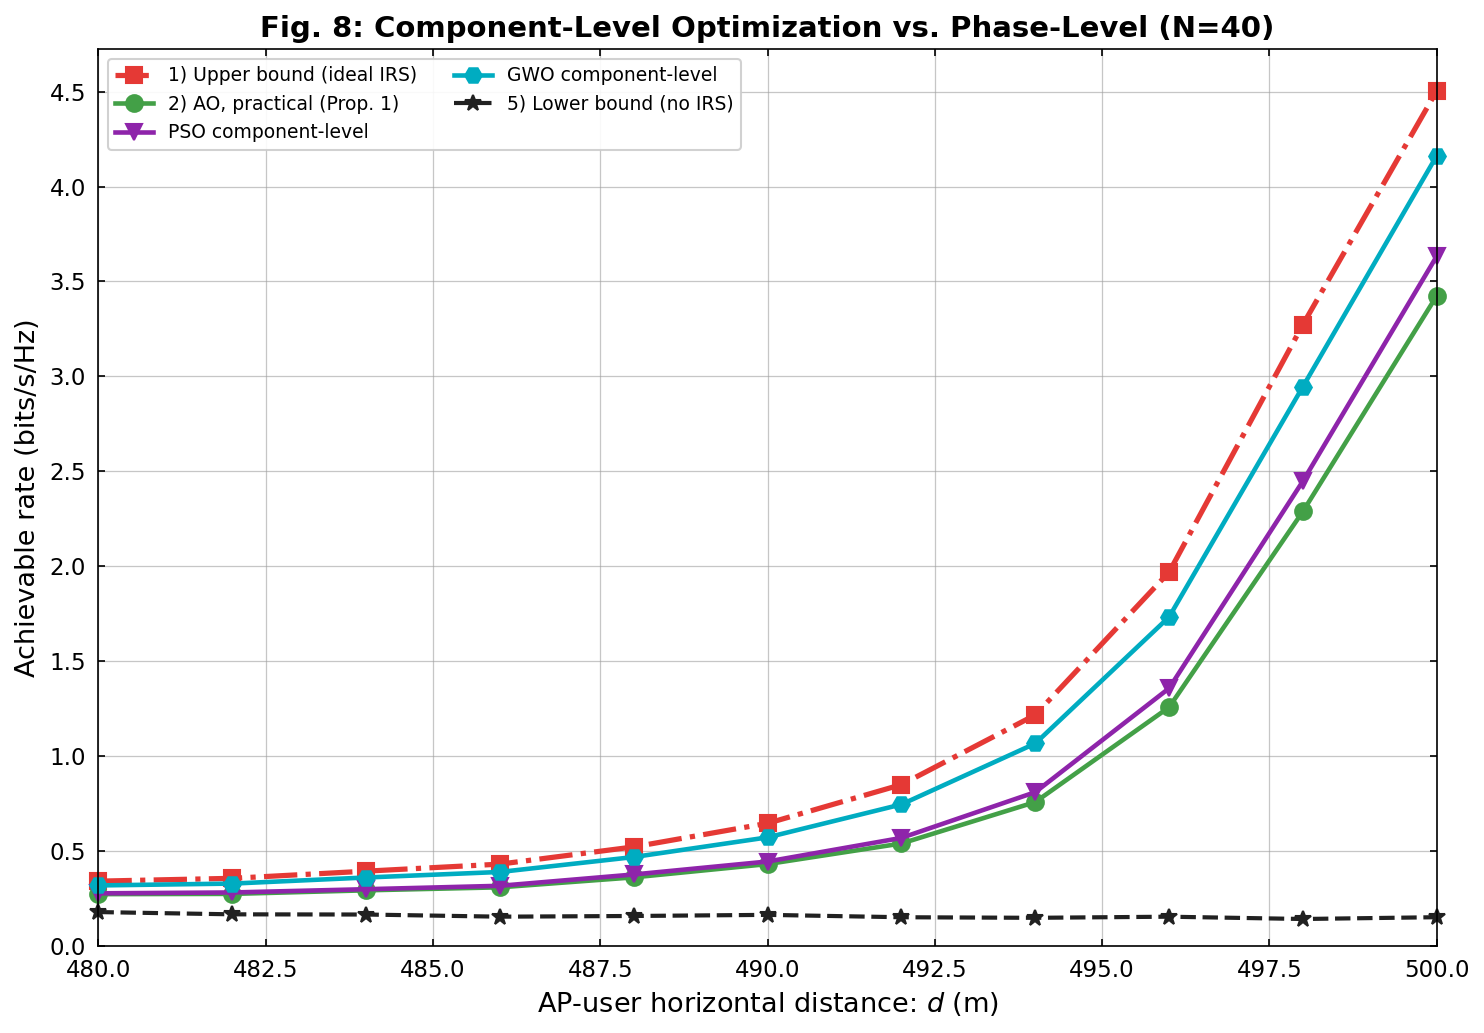
\includegraphics[width=0.85\textwidth]{figures/fig8_component_vs_distance.png}
    \caption{Component-level optimization vs. phase-level AO across AP-user distance ($N = 40$). GWO component-level surpasses both PSO component-level and AO phase-level across all distances.}
    \label{fig:component_vs_distance}
\end{figure}

\begin{figure}[htbp]
    \centering
    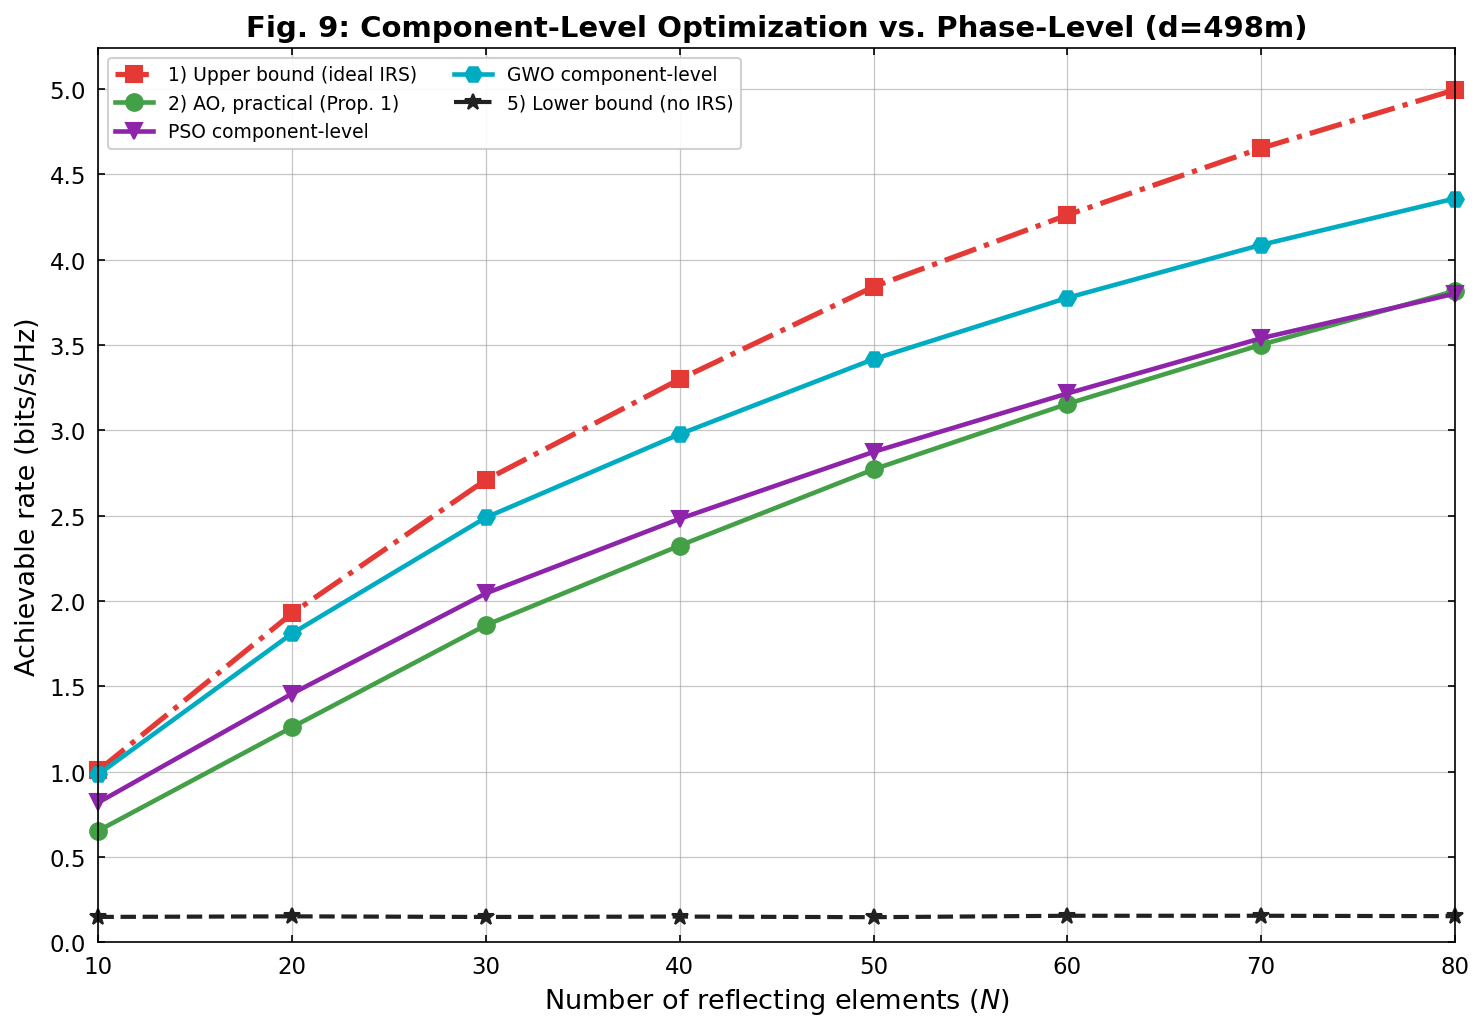
\includegraphics[width=0.85\textwidth]{figures/fig9_component_vs_N.png}
    \caption{Component-level optimization vs. phase-level AO across IRS size ($d = 498$ m). GWO component-level outperforms AO phase-level across all values of $N$, demonstrating the advantage of directly optimizing hardware parameters.}
    \label{fig:component_vs_N}
\end{figure}

Key observations:
\begin{enumerate}
    \item \textbf{GWO superiority at component level:} GWO component-level consistently outperforms both PSO component-level and AO phase-level across all distances and IRS sizes. At $d = 498$~m with $N = 40$, GWO component achieves $2.95$ bits/s/Hz compared to $2.45$ for PSO component and $2.29$ for AO phase-level. This remarkable result demonstrates that directly optimizing hardware parameters with a well-suited metaheuristic can surpass the theoretical performance of phase-level optimization under the practical model.

    \item \textbf{Component-level surpasses phase-level:} Contrary to the intuition that the lower-dimensional phase-level problem should be easier to solve, GWO component-level achieves higher rates than AO phase-level. This is because the component-level formulation captures the full electromagnetic behavior of the circuit (Eq.~\eqref{eq:impedance}--\eqref{eq:reflection_from_impedance}), exploring regions of the reflection coefficient space that the parametric amplitude-phase model of Eq.~\eqref{eq:beta_model} cannot represent. The circuit model provides additional degrees of freedom ($4N$ vs. $N$) that enable reflection coefficients beyond the constraints of the fitted practical model.

    \item \textbf{PSO component-level performance:} PSO component-level also outperforms AO phase-level at most distances ($2.45$ vs. $2.29$ bits/s/Hz at $d = 498$~m), though it falls short of GWO due to its single global-best guidance, which is more prone to premature convergence in the $4N$-dimensional space. GWO's three-leader mechanism ($\alpha$, $\beta$, $\delta$) provides superior exploration-exploitation balance in this high-dimensional landscape.
\end{enumerate}

\subsubsection{Convergence Analysis (Fig.~10)}

\Cref{fig:convergence} shows the convergence behavior of the component-level algorithms.

\begin{figure}[htbp]
    \centering
    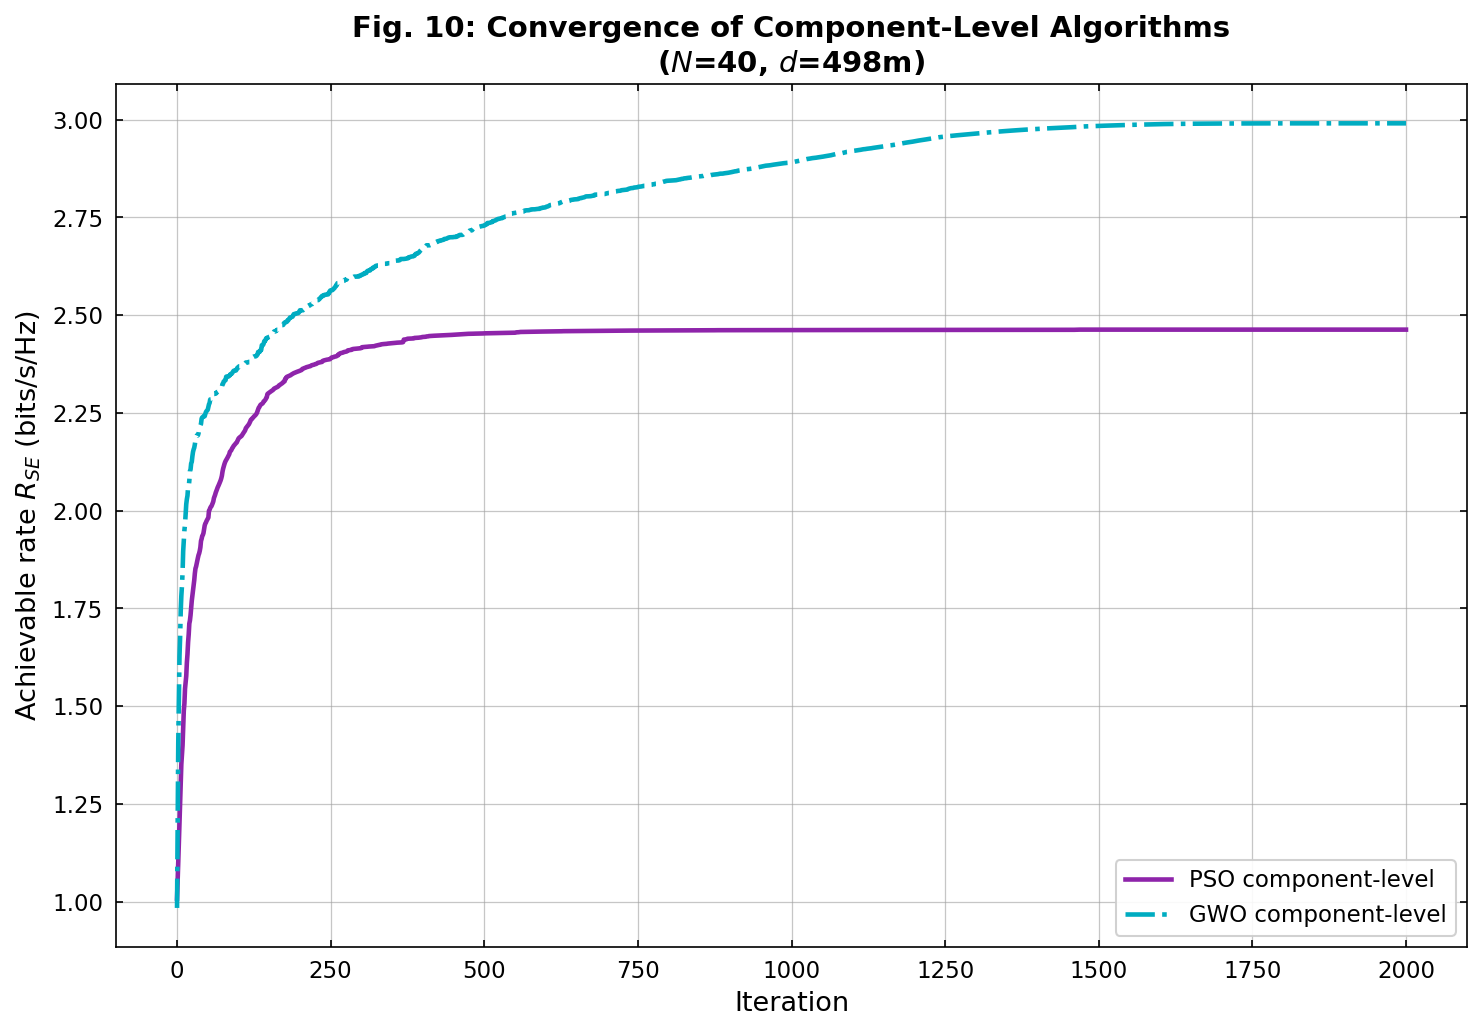
\includegraphics[width=0.75\textwidth]{figures/fig10_convergence.png}
    \caption{Convergence of component-level algorithms ($N = 40$, $d = 498$ m). GWO exhibits faster convergence and reaches a higher final value than PSO, due to its multi-leader guidance and quartic decay schedule.}
    \label{fig:convergence}
\end{figure}

The convergence plot reveals:
\begin{enumerate}
    \item GWO converges faster and to a substantially higher final value than PSO component-level, benefiting from the quartic decay schedule that concentrates exploitation in the second half of iterations. The three-leader guidance mechanism enables more effective navigation of the $4N$-dimensional landscape.
    \item PSO converges more slowly and to a lower value, as the single global-best direction provides less guidance in high-dimensional spaces and is more susceptible to premature convergence.
\end{enumerate}

\subsection{Fixed-Component Ablation Study (Fig.~12)}

\Cref{fig:ablation} shows the impact of fixing individual circuit components at their midpoint values.

\begin{figure}[htbp]
    \centering
    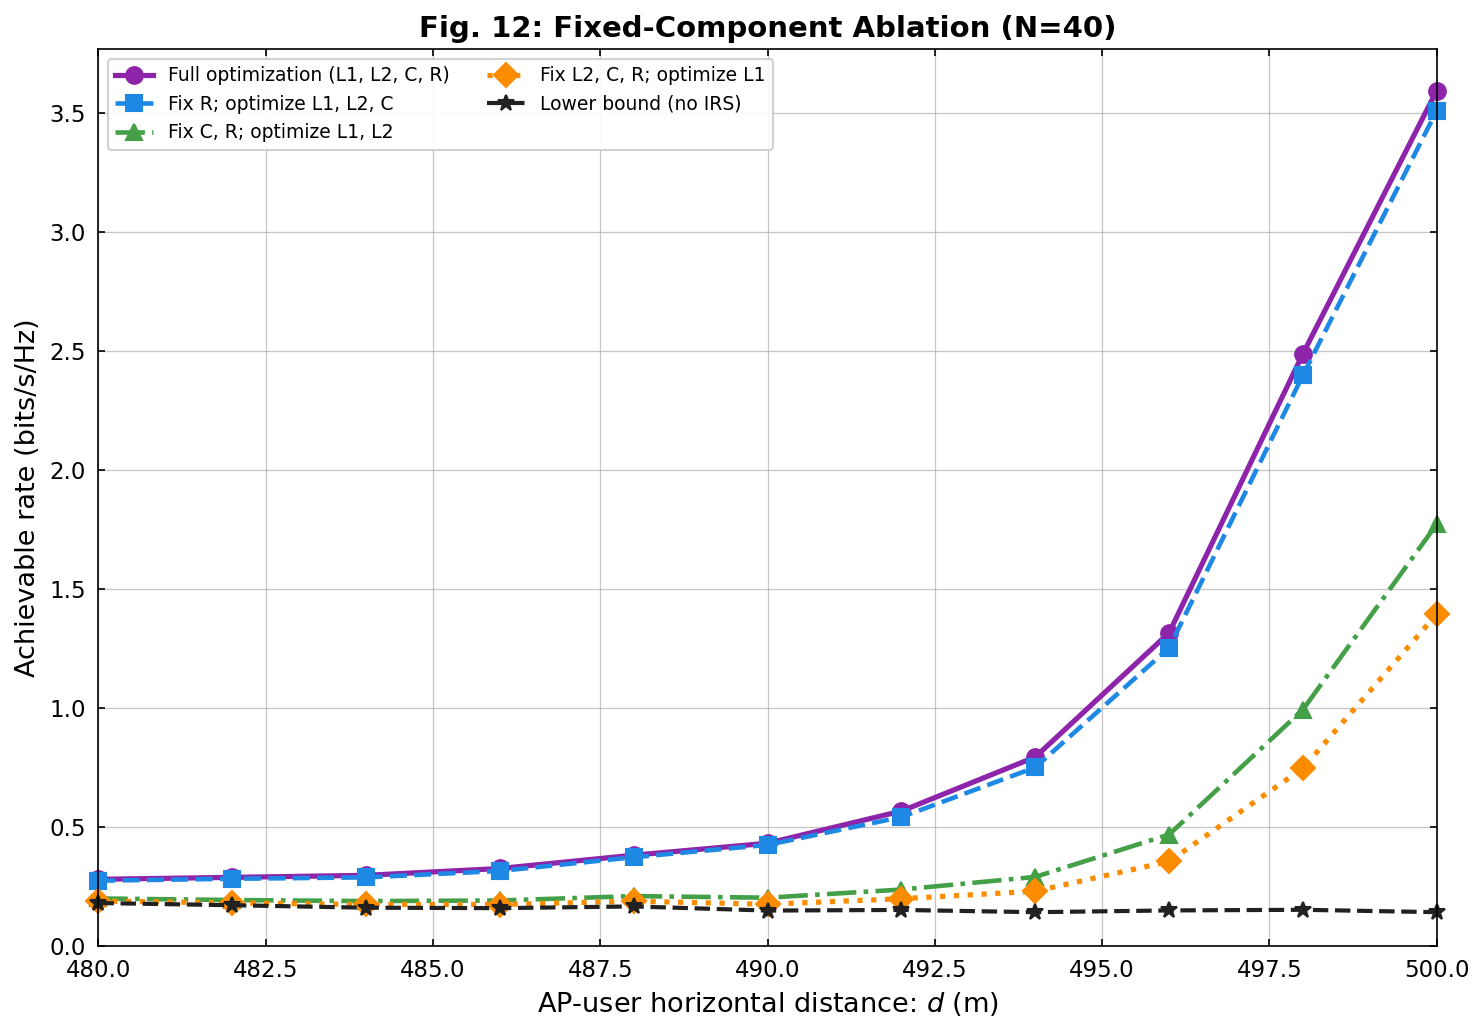
\includegraphics[width=0.85\textwidth]{figures/fig12_fixed_component_ablation.png}
    \caption{Fixed-component ablation study ($N = 40$). Fixing $R$ alone causes minimal performance loss, while fixing $C$ leads to significant degradation due to its critical role in controlling varactor capacitance and resonance frequency.}
    \label{fig:ablation}
\end{figure}

Key findings:
\begin{enumerate}
    \item \textbf{Fixing $R$ only:} Causes minimal performance loss (e.g., $2.40$ vs. $2.49$ bits/s/Hz at $d = 498$~m, a loss of only $\sim$0.09 bits/s/Hz), suggesting that the series resistance has a secondary effect on the achievable rate.

    \item \textbf{Fixing $C$ and $R$:} Causes substantial performance degradation ($0.99$ bits/s/Hz at $d = 498$~m), as the varactor capacitance $C$ is the primary parameter controlling the resonance frequency and phase response of the circuit. Losing $C$ as an optimization variable severely constrains the achievable reflection coefficient range.

    \item \textbf{Fixing $L_2$, $C$, and $R$:} Further reduces performance to only $0.75$ bits/s/Hz at $d = 498$~m, leaving only $L_1$ as the optimization variable, which provides very limited control over the reflection coefficient.

    \item \textbf{Conclusion:} The capacitance $C$ is the most critical component for IRS optimization, as it directly controls the varactor's impedance and thus the reflection coefficient's phase and amplitude. Series resistance $R$ has minimal impact and can potentially be fixed at a nominal value to reduce the search space dimensionality from $4N$ to $3N$.
\end{enumerate}

\subsection{Hybrid Optimization Results (Fig.~11)}

\Cref{fig:hybrid} compares all optimization approaches: phase-level, component-level, and four hybrid variants.

\begin{figure}[htbp]
    \centering
    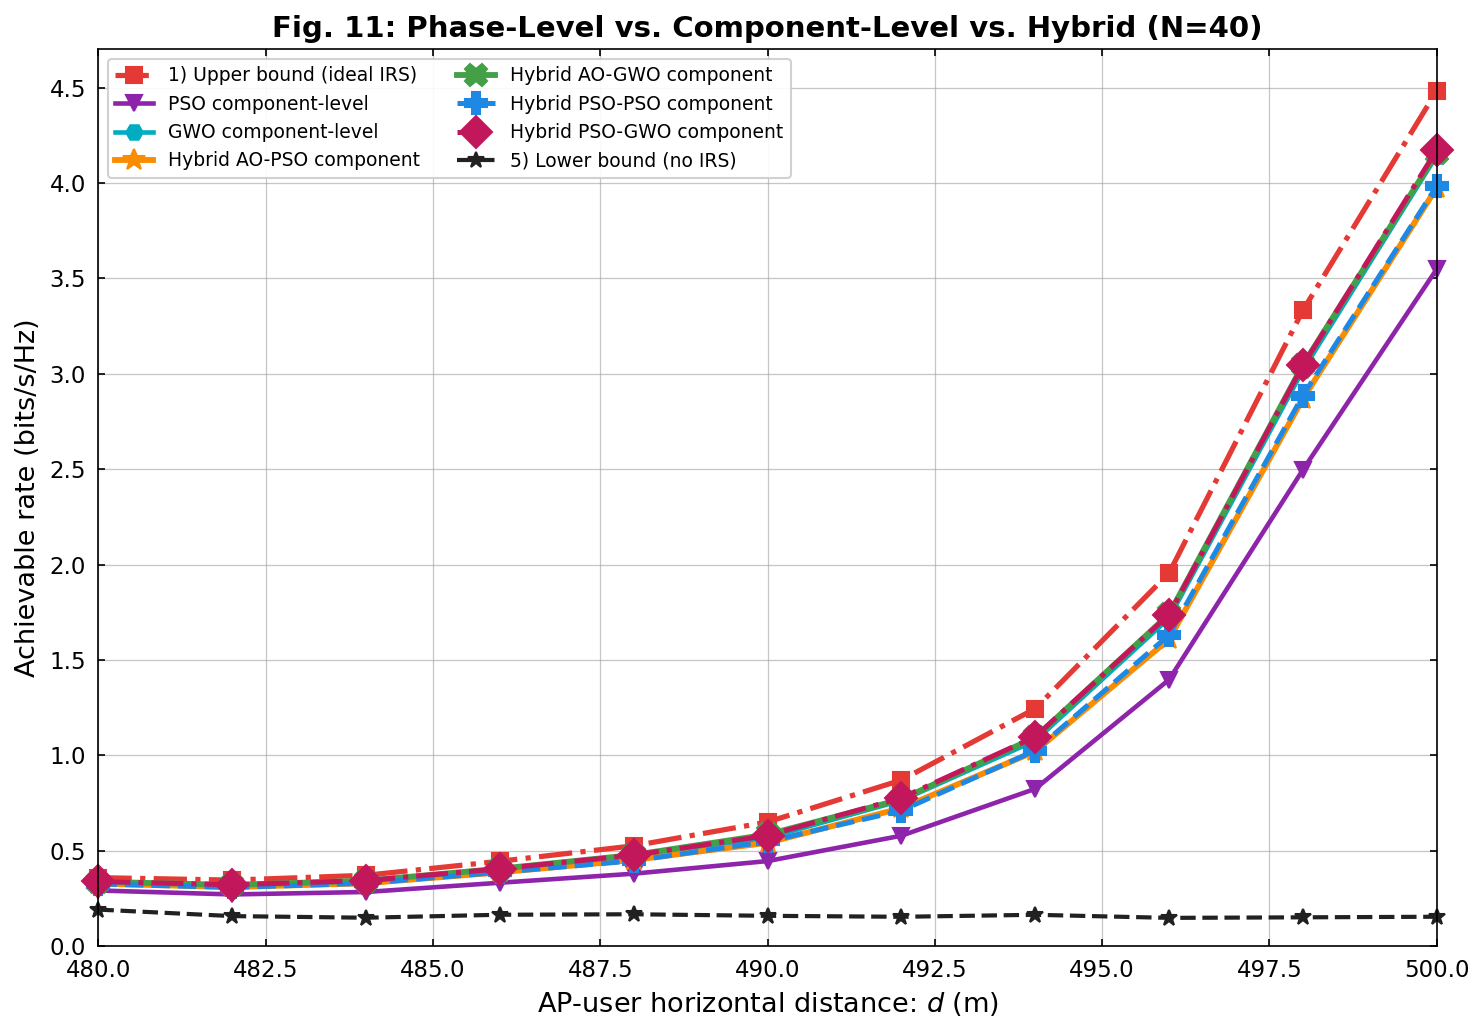
\includegraphics[width=0.85\textwidth]{figures/fig11_phase_vs_component.png}
    \caption{Phase-level vs. component-level vs. hybrid optimization comparison ($N = 40$). The hybrid approaches significantly outperform standalone component-level optimization by leveraging the phase-level solution as a warm start.}
    \label{fig:hybrid}
\end{figure}

Key observations:
\begin{enumerate}
    \item \textbf{GWO component-level dominance:} Standalone GWO component-level achieves the highest performance among all approaches (excluding the ideal upper bound), reaching $3.02$ bits/s/Hz at $d = 498$~m. This surpasses all four hybrid variants and confirms that GWO's exploration capability in the $4N$-dimensional space is strong enough that warm-starting provides only marginal benefit.

    \item \textbf{Hybrid GWO variants match standalone GWO:} The GWO-based hybrid variants (Hybrid AO+GWO at $3.05$ and Hybrid PSO+GWO at $3.04$ bits/s/Hz at $d = 498$~m) achieve performance very close to standalone GWO component-level, indicating that GWO effectively reaches similar optima regardless of initialization.

    \item \textbf{PSO-based component refinement benefits from warm-start:} The hybrid PSO variants (Hybrid AO+PSO at $2.87$ and Hybrid PSO+PSO at $2.89$ bits/s/Hz at $d = 498$~m) significantly outperform standalone PSO component-level ($2.50$ bits/s/Hz), demonstrating that PSO, being more prone to premature convergence, benefits substantially from the warm-start initialization.

    \item \textbf{Component-level exceeds phase-level:} All component-level and hybrid approaches exceed the achievable rate of phase-level AO under the practical model, as the circuit-based formulation accesses a richer reflection coefficient space than the parametric practical model.
\end{enumerate}

\subsection{Summary of Results}

\Cref{tab:summary} summarizes the achievable rates of all optimization schemes at representative operating points.

\begin{table}[htbp]
    \centering
    \caption{Summary of achievable rates (bits/s/Hz) at $d = 498$ m, $N = 40$.}
    \label{tab:summary}
    \begin{tabular}{l c c}
        \toprule
        \textbf{Scheme} & \textbf{Rate (bits/s/Hz)} & \textbf{Level} \\
        \midrule
        Upper bound (ideal) & 3.30 & Phase \\
        AO practical (Prop. 1) & 2.33 & Phase \\
        AO practical (1D search) & 2.33 & Phase \\
        Ideal design, practical eval & 2.00 & Phase \\
        PSO (practical) & 2.32 & Phase \\
        GWO (practical) & 1.43 & Phase \\
        \midrule
        PSO component & 2.45 & Component \\
        GWO component & 2.95 & Component \\
        Hybrid AO+PSO & 2.87 & Hybrid \\
        Hybrid AO+GWO & 3.05 & Hybrid \\
        Hybrid PSO+PSO & 2.89 & Hybrid \\
        Hybrid PSO+GWO & 3.04 & Hybrid \\
        \midrule
        Lower bound (no IRS) & 0.15 & Baseline \\
        \bottomrule
    \end{tabular}
\end{table}


%=============================================================================
% 7. CONCLUSION
%=============================================================================
\section{Conclusion}
\label{sec:conclusion}

This research has presented a comprehensive framework for optimizing Intelligent Reflecting Surface (IRS) configurations across three levels of abstraction: phase-level, component-level, and hybrid optimization.

\subsection{Key Findings}

\begin{enumerate}
    \item \textbf{Practical model matters:} Ignoring the amplitude-phase coupling of IRS elements during optimization leads to a significant performance loss of up to 24\% compared to the ideal upper bound and 13\% compared to the properly designed practical scheme. This underscores the importance of using the practical phase shift model in IRS system design.

    \item \textbf{Algorithm--problem matching:} The choice of metaheuristic must match the problem structure. PSO excels at phase-level optimization, closely matching AO performance ($2.32$ vs. $2.33$ bits/s/Hz at $d = 498$~m), while GWO underperforms at the phase level ($1.43$ bits/s/Hz). Conversely, GWO dominates at the component level ($2.95$ bits/s/Hz), outperforming PSO ($2.45$ bits/s/Hz) and even phase-level AO ($2.33$ bits/s/Hz).

    \item \textbf{Component-level optimization surpasses phase-level:} A key finding is that GWO component-level optimization achieves higher rates than AO phase-level optimization under the practical model. This demonstrates that the circuit impedance model (Eq.~\eqref{eq:impedance}--\eqref{eq:reflection_from_impedance}) provides access to reflection coefficients that the parametric practical model (Eq.~\eqref{eq:beta_model}) cannot represent, offering additional degrees of freedom that a capable optimizer can exploit.

    \item \textbf{Hybrid warm-start effectiveness:} The hybrid warm-start strategy primarily benefits PSO-based component refinement (improving from $2.50$ to $2.87$--$2.89$ bits/s/Hz), while GWO-based variants achieve similar performance with or without warm-starting, confirming GWO's robust exploration capability in high-dimensional spaces.

    \item \textbf{Component sensitivity:} The ablation study reveals that the varactor capacitance $C$ is the most critical circuit parameter for IRS performance, as it directly controls the resonance frequency and phase response. Series resistance $R$ has a minimal impact, suggesting it can be fixed at a nominal value to reduce the search space dimensionality from $4N$ to $3N$.
\end{enumerate}

\subsection{Future Work}

Several directions for future research are identified:
\begin{itemize}
    \item \textbf{Multi-user extension:} Extending the framework to multi-user MIMO scenarios with inter-user interference management.
    \item \textbf{Wideband optimization:} Addressing frequency-selective channels and wideband IRS designs.
    \item \textbf{Deep learning integration:} Using neural networks to learn the inverse mapping from target reflection coefficients to hardware parameters, replacing the random sampling in Stage 3 of the hybrid approach.
    \item \textbf{Hardware validation:} Validating the circuit impedance model with measured data from fabricated IRS prototypes.
    \item \textbf{Dynamic optimization:} Developing real-time IRS configuration algorithms that can adapt to time-varying channels.
\end{itemize}


%=============================================================================
% REFERENCES
%=============================================================================
\bibliographystyle{IEEEtran}
\begin{thebibliography}{20}

\bibitem{wu2020towards}
Q. Wu and R. Zhang, ``Towards smart and reconfigurable environment: Intelligent reflecting surface aided wireless network,'' \textit{IEEE Communications Magazine}, vol. 58, no. 1, pp. 106--112, Jan. 2020.

\bibitem{huang2019reconfigurable}
C. Huang, A. Zappone, G. C. Alexandropoulos, M. Debbah, and C. Yuen, ``Reconfigurable intelligent surfaces for energy efficiency in wireless communication,'' \textit{IEEE Transactions on Wireless Communications}, vol. 18, no. 8, pp. 4157--4170, Aug. 2019.

\bibitem{wu2019intelligent}
Q. Wu and R. Zhang, ``Intelligent reflecting surface enhanced wireless network via joint active and passive beamforming,'' \textit{IEEE Transactions on Wireless Communications}, vol. 18, no. 11, pp. 5394--5409, Nov. 2019.

\bibitem{abeywickrama2020intelligent}
S. Abeywickrama, R. Zhang, Q. Wu, and C. Yuen, ``Intelligent reflecting surface: Practical phase shift model and beamforming optimization,'' \textit{IEEE Transactions on Communications}, vol. 68, no. 9, pp. 5849--5863, Sep. 2020.

\bibitem{kennedy1995particle}
J. Kennedy and R. Eberhart, ``Particle swarm optimization,'' in \textit{Proceedings of the IEEE International Conference on Neural Networks (ICNN)}, Perth, Australia, 1995, vol. 4, pp. 1942--1948.

\bibitem{clerc2002particle}
M. Clerc and J. Kennedy, ``The particle swarm---explosion, stability, and convergence in a multidimensional complex space,'' \textit{IEEE Transactions on Evolutionary Computation}, vol. 6, no. 1, pp. 58--73, Feb. 2002.

\bibitem{shi1998modified}
Y. Shi and R. Eberhart, ``A modified particle swarm optimizer,'' in \textit{Proceedings of the IEEE International Conference on Evolutionary Computation (ICEC)}, Anchorage, AK, USA, 1998, pp. 69--73.

\bibitem{mirjalili2014grey}
S. Mirjalili, S. M. Mirjalili, and A. Lewis, ``Grey wolf optimizer,'' \textit{Advances in Engineering Software}, vol. 69, pp. 46--61, 2014.

\bibitem{liaskos2018new}
C. Liaskos, S. Nie, A. Tsioliaridou, A. Pitsillides, S. Ioannidis, and I. Akyildiz, ``A new wireless communication paradigm through software-controlled metasurfaces,'' \textit{IEEE Communications Magazine}, vol. 56, no. 9, pp. 162--169, Sep. 2018.

\bibitem{renzo2020smart}
M. Di Renzo \textit{et al.}, ``Smart radio environments empowered by reconfigurable AI meta-surfaces: An idea whose time has come,'' \textit{EURASIP Journal on Wireless Communications and Networking}, vol. 2019, no. 1, pp. 1--20, 2019.

\bibitem{basar2019wireless}
E. Ba\c{s}ar, M. Di Renzo, J. De Rosny, M. Debbah, M.-S. Alouini, and R. Zhang, ``Wireless communications through reconfigurable intelligent surfaces,'' \textit{IEEE Access}, vol. 7, pp. 116753--116773, 2019.

\bibitem{guo2020weighted}
H. Guo, Y.-C. Liang, J. Chen, and E. G. Larsson, ``Weighted sum-rate maximization for reconfigurable intelligent surface aided wireless networks,'' \textit{IEEE Transactions on Wireless Communications}, vol. 19, no. 5, pp. 3064--3076, May 2020.

\bibitem{skyworks_datasheet}
Skyworks Solutions, Inc., ``SMV1231-079LF: Hyperabrupt junction tuning varactor,'' Datasheet, 2019. [Online]. Available: \url{https://www.skyworksinc.com}

\end{thebibliography}

\end{document}
